% Options for packages loaded elsewhere
\PassOptionsToPackage{unicode}{hyperref}
\PassOptionsToPackage{hyphens}{url}
\PassOptionsToPackage{dvipsnames,svgnames,x11names}{xcolor}
%
\documentclass[
  letterpaper,
  DIV=11,
  numbers=noendperiod]{scrartcl}

\usepackage{amsmath,amssymb}
\usepackage{iftex}
\ifPDFTeX
  \usepackage[T1]{fontenc}
  \usepackage[utf8]{inputenc}
  \usepackage{textcomp} % provide euro and other symbols
\else % if luatex or xetex
  \usepackage{unicode-math}
  \defaultfontfeatures{Scale=MatchLowercase}
  \defaultfontfeatures[\rmfamily]{Ligatures=TeX,Scale=1}
\fi
\usepackage{lmodern}
\ifPDFTeX\else  
    % xetex/luatex font selection
\fi
% Use upquote if available, for straight quotes in verbatim environments
\IfFileExists{upquote.sty}{\usepackage{upquote}}{}
\IfFileExists{microtype.sty}{% use microtype if available
  \usepackage[]{microtype}
  \UseMicrotypeSet[protrusion]{basicmath} % disable protrusion for tt fonts
}{}
\makeatletter
\@ifundefined{KOMAClassName}{% if non-KOMA class
  \IfFileExists{parskip.sty}{%
    \usepackage{parskip}
  }{% else
    \setlength{\parindent}{0pt}
    \setlength{\parskip}{6pt plus 2pt minus 1pt}}
}{% if KOMA class
  \KOMAoptions{parskip=half}}
\makeatother
\usepackage{xcolor}
\setlength{\emergencystretch}{3em} % prevent overfull lines
\setcounter{secnumdepth}{5}
% Make \paragraph and \subparagraph free-standing
\ifx\paragraph\undefined\else
  \let\oldparagraph\paragraph
  \renewcommand{\paragraph}[1]{\oldparagraph{#1}\mbox{}}
\fi
\ifx\subparagraph\undefined\else
  \let\oldsubparagraph\subparagraph
  \renewcommand{\subparagraph}[1]{\oldsubparagraph{#1}\mbox{}}
\fi


\providecommand{\tightlist}{%
  \setlength{\itemsep}{0pt}\setlength{\parskip}{0pt}}\usepackage{longtable,booktabs,array}
\usepackage{calc} % for calculating minipage widths
% Correct order of tables after \paragraph or \subparagraph
\usepackage{etoolbox}
\makeatletter
\patchcmd\longtable{\par}{\if@noskipsec\mbox{}\fi\par}{}{}
\makeatother
% Allow footnotes in longtable head/foot
\IfFileExists{footnotehyper.sty}{\usepackage{footnotehyper}}{\usepackage{footnote}}
\makesavenoteenv{longtable}
\usepackage{graphicx}
\makeatletter
\def\maxwidth{\ifdim\Gin@nat@width>\linewidth\linewidth\else\Gin@nat@width\fi}
\def\maxheight{\ifdim\Gin@nat@height>\textheight\textheight\else\Gin@nat@height\fi}
\makeatother
% Scale images if necessary, so that they will not overflow the page
% margins by default, and it is still possible to overwrite the defaults
% using explicit options in \includegraphics[width, height, ...]{}
\setkeys{Gin}{width=\maxwidth,height=\maxheight,keepaspectratio}
% Set default figure placement to htbp
\makeatletter
\def\fps@figure{htbp}
\makeatother
\newlength{\cslhangindent}
\setlength{\cslhangindent}{1.5em}
\newlength{\csllabelwidth}
\setlength{\csllabelwidth}{3em}
\newlength{\cslentryspacingunit} % times entry-spacing
\setlength{\cslentryspacingunit}{\parskip}
\newenvironment{CSLReferences}[2] % #1 hanging-ident, #2 entry spacing
 {% don't indent paragraphs
  \setlength{\parindent}{0pt}
  % turn on hanging indent if param 1 is 1
  \ifodd #1
  \let\oldpar\par
  \def\par{\hangindent=\cslhangindent\oldpar}
  \fi
  % set entry spacing
  \setlength{\parskip}{#2\cslentryspacingunit}
 }%
 {}
\usepackage{calc}
\newcommand{\CSLBlock}[1]{#1\hfill\break}
\newcommand{\CSLLeftMargin}[1]{\parbox[t]{\csllabelwidth}{#1}}
\newcommand{\CSLRightInline}[1]{\parbox[t]{\linewidth - \csllabelwidth}{#1}\break}
\newcommand{\CSLIndent}[1]{\hspace{\cslhangindent}#1}

\KOMAoption{captions}{tableheading}
\makeatletter
\makeatother
\makeatletter
\makeatother
\makeatletter
\@ifpackageloaded{caption}{}{\usepackage{caption}}
\AtBeginDocument{%
\ifdefined\contentsname
  \renewcommand*\contentsname{Table of contents}
\else
  \newcommand\contentsname{Table of contents}
\fi
\ifdefined\listfigurename
  \renewcommand*\listfigurename{List of Figures}
\else
  \newcommand\listfigurename{List of Figures}
\fi
\ifdefined\listtablename
  \renewcommand*\listtablename{List of Tables}
\else
  \newcommand\listtablename{List of Tables}
\fi
\ifdefined\figurename
  \renewcommand*\figurename{Figure}
\else
  \newcommand\figurename{Figure}
\fi
\ifdefined\tablename
  \renewcommand*\tablename{Table}
\else
  \newcommand\tablename{Table}
\fi
}
\@ifpackageloaded{float}{}{\usepackage{float}}
\floatstyle{ruled}
\@ifundefined{c@chapter}{\newfloat{codelisting}{h}{lop}}{\newfloat{codelisting}{h}{lop}[chapter]}
\floatname{codelisting}{Listing}
\newcommand*\listoflistings{\listof{codelisting}{List of Listings}}
\makeatother
\makeatletter
\@ifpackageloaded{caption}{}{\usepackage{caption}}
\@ifpackageloaded{subcaption}{}{\usepackage{subcaption}}
\makeatother
\makeatletter
\@ifpackageloaded{tcolorbox}{}{\usepackage[skins,breakable]{tcolorbox}}
\makeatother
\makeatletter
\@ifundefined{shadecolor}{\definecolor{shadecolor}{rgb}{.97, .97, .97}}
\makeatother
\makeatletter
\makeatother
\makeatletter
\makeatother
\ifLuaTeX
  \usepackage{selnolig}  % disable illegal ligatures
\fi
\IfFileExists{bookmark.sty}{\usepackage{bookmark}}{\usepackage{hyperref}}
\IfFileExists{xurl.sty}{\usepackage{xurl}}{} % add URL line breaks if available
\urlstyle{same} % disable monospaced font for URLs
\hypersetup{
  pdftitle={Probability Theory on General Spaces},
  pdfauthor={Michael Betancourt},
  colorlinks=true,
  linkcolor={blue},
  filecolor={Maroon},
  citecolor={Blue},
  urlcolor={Blue},
  pdfcreator={LaTeX via pandoc}}

\title{Probability Theory on General Spaces}
\author{Michael Betancourt}
\date{July 2023}

\begin{document}
\maketitle
\ifdefined\Shaded\renewenvironment{Shaded}{\begin{tcolorbox}[interior hidden, boxrule=0pt, sharp corners, frame hidden, breakable, borderline west={3pt}{0pt}{shadecolor}, enhanced]}{\end{tcolorbox}}\fi

\renewcommand*\contentsname{Table of contents}
{
\hypersetup{linkcolor=}
\setcounter{tocdepth}{3}
\tableofcontents
}
Previously in
\href{https://betanalpha.github.io/assets/chapters_html/probability_on_finite_sets.html}{Chapter
One} we introduced measure and probability theory over sets with only a
finite number of elements. We saw in
\href{https://betanalpha.github.io/assets/chapters_html/spaces.html}{Chapter
Two}, however, that many of the most mathematical spaces we encounter in
practical applications, like the integers and the real line, feature not
a finite number of elements but rather countably infinite and even
uncountably infinite numbers of elements. Unfortunately extending
measure and probability theory to more general spaces like these is not
always straightforward.

In this chapter we will investigate the difficulties in defining measure
and probability theory on general mathematical spaces, with a focus on
concepts instead of technical details. We will first discuss why
measures allocated to individual elements does not, in general, provide
enough information to define a consistent allocation for all subsets.
Then we will consider how certain pathological subsets on some spaces
can obstruct consistent allocations over the full power set, and how we
can systematically remove these obstructions in practice. Finally we
will present the most general form of measure and probability theory
that can be applied to any mathematical space and then discuss some
common applications.

\hypertarget{allocation-over-elements}{%
\section{Allocation Over Elements}\label{allocation-over-elements}}

Recall that in
\href{https://betanalpha.github.io/assets/chapters_html/probability_on_finite_sets.html}{Chapter
One} we first defined measures and probability distributions as
allocations over the individual elements in a finite set. More formally
we were able to define a measure as a function that mapped each element
to its allocation of the total measure, \begin{alignat*}{6}
\mu :\; & X & &\rightarrow& \; & [0, \infty] &
\\
& x & &\mapsto& & \mu(x) &.
\end{alignat*}

This element-wise allocation then allowed us to define the measure
allocated to subsets. In particular the measure allocated to a subset
\(\mathsf{x} \subset X\) was unambiguously determined by summing up the
measures allocated to the included elements, \[
\mu(\mathsf{x}) = \sum_{x \in \mathsf{x}} \mu(x).
\] On finite spaces this construction gives us a \emph{consistent}
allocation in the sense that the total measure is always preserved no
matter how we might decompose the ambient set into subsets.

Conveniently this construction does extend to spaces with countably
infinite numbers of elements, such as the integers. In these spaces
every subset contains at most a countably infinite number of elements
and sums of measures will always converge to well-defined values.
Element-wise measure allocations on finite and countably infinite spaces
are also known as \textbf{mass functions}, with element-wise probability
allocations also known as \textbf{probability mass functions}.

Unfortunately the element-wise construction does not extend any further.
Once we consider spaces with uncountably infinite numbers of elements,
such as the real numbers, we have to confront subsets with uncountably
infinite numbers of elements where sums start to misbehave.

Consider for example a subset \(\mathsf{x}\) where each of the included
elements has been allocated exactly zero measure. If \(\mathsf{x}\)
contains only a finite or countably infinite number of elements then the
sum of these zero measures \emph{always} yields zero.

When \(\mathsf{x}\) contains an uncountably infinite number of elements,
however, the sum of the individual element measures is not necessarily
zero. In fact it can give \emph{any} value between zero and infinity;
uncountably infinite spaces have so many elements that we can very much
get something from nothing!

Ultimately this means that on general spaces the allocation of measure
to individual elements \emph{does not provide enough information} to
uniquely determine what measure should be allocated to every combination
of those elements. In order to completely define a measure we need to
specify what those subset allocations are ourselves.

\hypertarget{allocation-over-all-subsets}{%
\section{Allocation Over All
Subsets}\label{allocation-over-all-subsets}}

In
\href{https://betanalpha.github.io/assets/chapters_html/probability_on_finite_sets.html}{Chapter
One} we also considered defining a measure by specifying allocations to
each subset in the power set, \begin{alignat*}{6}
\mu :\; & 2^{X} & &\rightarrow& \; & [0, \infty] &
\\
& \mathsf{x} & &\mapsto& & \mu(\mathsf{x}) &.
\end{alignat*} Importantly these subsets allocations needed to be
consistent with each other to match the behavior of those derived from
individual element allocations. For any finite collection of disjoint
subsets we should have \[
\mu( \cup_{i = 1}^{I} \mathsf{x} )
=
\sum_{i = 1}^{I} \mu( \mathsf{x}_{i}).
\]

For finite spaces this construction is excessive; the subset allocations
contain an abundance of redundant information. Because we also can
derive subset allocations from element-wise allocations on countably
infinite spaces, this construction is unnecessary there as well.

On the other hand at least some subset allocation is strictly necessary
for fully defining measures on uncountably infinite spaces, and hence
mathematical spaces in general. The only question is whether or not
\emph{consistent} subset allocations are even possible on these more
sophisticated spaces.

\hypertarget{consistent-allocations}{%
\subsection{Consistent Allocations}\label{consistent-allocations}}

Before answering this question let's take a second to define exactly
what kind of consistency we need. Because finite spaces feature only a
finite number of subsets we only ever have to consider the consistency
of a finite collection of subsets at a time. More formally if \[
\{ \mathsf{x}_{1}, \ldots, \mathsf{x}_{i}, \ldots, \mathsf{x}_{I} \}
\] is any finite collection of disjoint subsets, \[
\mathsf{x}_{i} \cup \mathsf{x}_{i' \ne i} = \emptyset,
\] then a consistent measure should give \[
\mu( \cup_{i = 1}^{I} \mathsf{x} )
=
\sum_{i = 1}^{I} \mu( \mathsf{x}_{i}).
\] Regardless of how many elements the ambient space contains,
consistency of a measure over any finite collection of subsets is known
as \textbf{finite additivity}.

More general spaces can feature infinitely many subsets, and hence
different possible notions of additive consistency. For example on a
countably infinite space the subset allocations derived from a mass
function are consistent across countably infinite collections of
subsets. If \[
\{ \mathsf{x}_{1}, \ldots, \mathsf{x}_{i}, \ldots \}
\] is any countably infinite collection of disjoint subsets with with \[
\mathsf{x}_{i} \cup \mathsf{x}_{i' \ne i} = \emptyset
\] then \[
\mu( \cup_{i} \mathsf{x} )
=
\sum_{i} \mu( \mathsf{x}_{i}).
\] This is known as \textbf{countable additivity}.

The question is then whether measures with finite additivity are
sufficiently useful for practical application or if we need to consider
countably additive measures, let alone measures that might be additive
over even larger collections of subsets.

For example a common problem that arises is practice is reconstructing
the measure allocated to a general subset from the measures allocated to
particularly nice subsets that are easier with which to work. If we
could always decompose a generic subset into the disjoint union of a
finite number of nice subsets then finite additivity would be sufficient
for this task. On the other hand if we could decompose a generic subset
into the disjoint union of only a countably infinite number of nice
subsets then countable additivity would be sufficient. Potentially some
subsets might be decomposable only into an uncountably infinite number
of subsets in which case we would need even stronger notions of
additivity!

Fortunately for us we don't have to go to that last extreme. In turns
out that on most spaces that we'll encounter in practice, and typical
notions of ``nice'' subsets, countable additivity is sufficient for
reconstructing the measure allocated to more general subsets.

To demonstrate let's consider the two-dimensional real plane
\(\mathbb{R}^{2}\) and a measure that is partially defined through it's
allocations to \textbf{rectangular} subsets
(Figure~\ref{fig-disk-decomposition}). In general a non-rectangular
subset, in this case a disk, can be crudely approximated by a single
rectangular subset. The disk can be approximated more precisely as the
disjoint union of many different rectangular subsets, but that will
never exact reconstruct the disk. Only when we incorporate a countably
infinite number of rectangular subsets can be reconstruct the disk
without any error.

\begin{figure}

{\centering 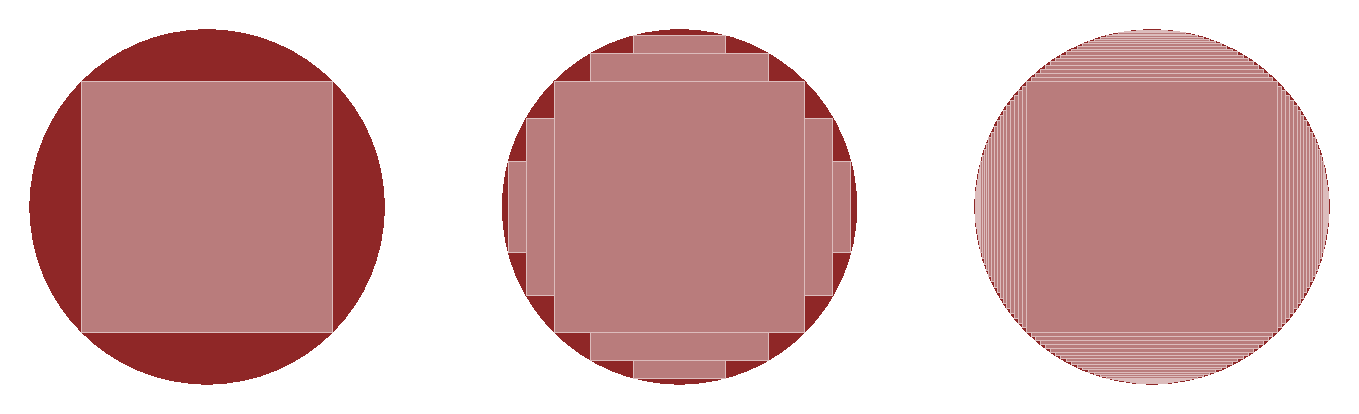
\includegraphics[width=0.9\textwidth,height=\textheight]{figures/disk_decomposition/disk_decomposition.pdf}

}

\caption{\label{fig-disk-decomposition}On a two-dimensional real plane
\(\mathbb{R}^{2}\) a non-rectangular disc can be approximated, but not
exactly reconstructed, by the finite union of different rectangular
subsets. In order to exactly reconstruct a non-rectangular subset we
need to include a countably infinite number of rectangular subsets. If
measures are countably additive then we can use this decomposition to
reconstruct the measure allocated to the disk by adding up the measures
allocated to the infinitely many rectangular subsets in the
reconstruction.}

\end{figure}

Ultimately countable additive measures give us the mathematical
flexibility we need for many practical applications.

\hypertarget{sub-additivity-and-super-additivity}{%
\subsection{Sub-Additivity and
Super-Additivity}\label{sub-additivity-and-super-additivity}}

Ideally we would be able to define measures that are additive over any
countably infinite collection of disjoint subsets on any space.
Unfortunately mathematics is not always kind, and many seemingly
well-behaved space feature pathological subsets that obstruct countable
additivity.

Specifically many uncountably infinite spaces feature disjoint subsets
that will always behave \textbf{sub-additivity}, \begin{align*}
\mathsf{x}_{1} \cup \mathsf{x}_{2} &= \emptyset
\\
\mu( \mathsf{x}_{1} \cup \mathsf{x}_{2} )
&<
\mu( \mathsf{x}_{1}) + \mu( \mathsf{x}_{2} )
\end{align*} no matter how we try to define the allocation! In other
words the power set will always be infiltrated by certain subsets that
are always less than the sum of their parts and obstruct a consistent
definition of measure.

At the same time we can generally show that there exist disjoint subsets
that are \textbf{super-additive}, \begin{align*}
\mathsf{x}_{1} \cup \mathsf{x}_{2} &= \emptyset
\\
\mu( \mathsf{x}_{1} \cup \mathsf{x}_{2} )
&>
\mu( \mathsf{x}_{1}) + \mu( \mathsf{x}_{2} ).
\end{align*} In other words if the measure allocated to these subsets
and the measure allocated to their union then we will always appear to
end up with measure than what had been initially allocated.

What makes these pathological subsets even more awkward is that we can't
actually construct them from explicit conditions. Given typical
assumptions about infinity all we can do is prove that these subsets
exist. These phantom subsets are known as \textbf{non-constructive}
objects.

That said because the misbehaving subsets are non-constructive we don't
really need to consider them in any practical application of measure
theory. If we could consistently filter them out of the full power set
then we would be able to define consistent measures over the remaining
subsets, and that would be sufficient for any practical application.

\hypertarget{sigma-algebras}{%
\section{\texorpdfstring{\(\sigma\)-Algebras}{\textbackslash sigma-Algebras}}\label{sigma-algebras}}

Because the term ``\(\sigma\)-algebra'' is often thrown around in
measure and probability theory without much explanation it is often seen
as an impenetrable concept that defies explanation. In reality, however,
\(\sigma\)-algebra are simply a way to consistently filter out subsets
from the power set.

\hypertarget{filtering-subsets}{%
\subsection{Filtering Subsets}\label{filtering-subsets}}

We can always filter the power set by removing certain subsets. The
difficultly is ensuring that no application of the three set operations
would ever lead us back to the excised subsets and reveal a ``hole'' in
the remaining collection of subsets. In other words we need our filtered
collection of subsets to be \emph{closed} under the three set operations
so that there is no risk of accidentally recreating a subset outside of
the collection.

In particular if the subset \(\mathsf{x} \subset X\) is in our filtered
collection then so too should be the complement \(\mathsf{x}^{c}\). If
this is true then anytime we apply the complement operator to a subset
in our collection we are guaranteed to always see another subset in our
collection.

Similarly for every pair of subsets \(\mathsf{x}_{1} \subset X\) and
\(\mathsf{x}_{1} \subset X\) in a filtered collection the union
\(\mathsf{x}_{1} \cup \mathsf{x}_{2}\) and intersection
\(\mathsf{x}_{1} \cap \mathsf{x}_{2}\) should also be in the collection.
In order to ensure closure under repeated applications of the union and
intersection operators we need the union and intersection of any
countably infinite sequences of subsets to also be in the filtered
collection.

A \textbf{\(\sigma\)-algebra} is any collection of subsets that is
closed under complements, countable unions, and countable intersections.
In other words a \(\sigma\)-algebra is just any consistent filtering of
the power set. I will use a calligraphic font to refer to
\(\sigma\)-algebras so that if \(X\) is a space then
\(\mathcal{X} \subset 2^{X}\) will denote a \(\sigma\)-algebra defined
on that space.

A set equipped with a \(\sigma\)-algebra, \((X, \mathcal{X})\) is known
as a \textbf{measurable space}. I will refer to \(X\) as the
\textbf{ambient set}, or the \textbf{ambient space} if it is also
equipped with additional structure. Similarly the elements of a
\(\sigma\)-algebra are known as \textbf{measurable sets} while any
subsets in the power set but not in the \(\sigma\)-algebra are referred
to as \textbf{non-measurable} subsets.

When non-measurable subsets are misbehaving subsets they reveals the
subtle, and often counterintuitive, pathologies inherent to that space.
By working with \(sigma\)-algebras directly we can avoid these awkward
pathologies entirely.

\hypertarget{generating-sigma-algebras}{%
\subsection{\texorpdfstring{Generating
\(\sigma\)-Algebras}{Generating \textbackslash sigma-Algebras}}\label{generating-sigma-algebras}}

Now that we've defined how a consistent sub-collection of subsets
behaves we need to consider how to construct these \(\sigma\)-algebras
in practice. One particularly useful way to build up \(\sigma\)-algebras
is to \emph{generate} them by repeatedly applying the three set
operations to an initial collection of subsets.

For example consider an initial collection of two subsets \[
\{ \mathsf{x}_1, \mathsf{x}_2 \}.
\] Applying the complement operator gives us two subsets that fall
outside of the initial collection, \[
\{ \mathsf{x}_1^c, \mathsf{x}_2^c \},
\] Similarly applying the union operator gives \[
\{ \mathsf{x}_1 \cup \mathsf{x}_2 \}
\] while applying the intersection operator gives \[
\{ \mathsf{x}_1 \cap \mathsf{x}_2 \}.
\] To ensure closure we have to add \emph{all} of these subsets to our
initial collection, \[
\{ \mathsf{x}_1, \mathsf{x}_2, \mathsf{x}_1^c, \mathsf{x}_2^c,
   \mathsf{x}_1 \cup \mathsf{x}_2, \mathsf{x}_1 \cap \mathsf{x}_2 \}.
\] At this point we iterate, applying the complement operator to every
subset and the union and intersection operators to every finite and
countably infinite sub-collection of subsets to generate an even larger
collection of subsets. When the set operations no longer return new
subsets the final collection of subsets defines a \(\sigma\)-algebra.

A convenient feature of this procedure is that if we start with a
collection of constructive subsets then we will \emph{always} end up
with a \(\sigma\)-algebra that is free of any non-constructive subsets
and their pathological behaviors. To ensure that we don't filter out any
well-behaved subsets in the process we just have to make sure that our
initial collection is sufficiently large.

Conveniently when working on a topological space we already have a
natural collection of subsets that we can use to generate a
\(\sigma\)-algebra -- the defining topology itself! The
\(\sigma\)-algebra generated by repeatedly applying all three set
operations to the subsets in a topology is known as a \textbf{Borel}
\(\sigma\)-algebra. In other words a Borel \(\sigma\)-algebra is the
unique \(\sigma\)-algebra comprised of all of the open and closed
subsets.

Every space that we will consider in this book will be a topological
space. Consequently we can always use the corresponding Borel
\(\sigma\)-algebra to remove any undesired subsets that would obstruct
the definition of a consistent measures and probability distributions.
Indeed Borel \(\sigma\)-algebras are so common that they are often take
for granted, with any reference to a ``measurable space'' implicitly
assuming a topological space and its corresponding Borel
\(\sigma\)-algebras to filter out any inconsistent behavior.

For example finite and countably infinite spaces are almost always
equipped with discrete topologies. Because discrete topologies contain
all of the atomic sets the \(\sigma\)-algebras derived from them will
always be the full power set. There are no pathological behaviors that
we have to avoid in these cases.

On the the other hand the Borel \(\sigma\)-algebra derived from the
topology that defines the real line filters out all of the
non-constructive subsets and their undesired behaviors. This results in
a \(\sigma\)-algebra that is strictly smaller than the full power set of
the real line.

A Borel \(\sigma\)-algebra is sufficient for removing any
counterintuitive behavior from a topological space but in more technical
mathematical work there are circumstances where slightly larger
\(\sigma\)-algebras may be more convenient. In more applied practice we
can safely assume a Borel \(\sigma\)-algebra or any extension that might
be needed to avoid any technical problems.

\hypertarget{measures-and-probability-distributions}{%
\section{Measures and Probability
Distributions}\label{measures-and-probability-distributions}}

With all of that work we are finally ready to define a theory for
allocating any conserved, but not necessarily finite, quantity across a
general mathematical space.

\hypertarget{formal-definitions}{%
\subsection{Formal Definitions}\label{formal-definitions}}

A \textbf{measure} on any measurable space \((X, \mathcal{X})\) is a
function from the \(\sigma\)-algebra \(\mathcal{X}\) to the extended
positive real line, \begin{alignat*}{6}
\mu :\; & \mathcal{X} & &\rightarrow& \; & [0, \infty] &
\\
& \mathsf{x} & &\mapsto& & \mu(\mathsf{x}) &,
\end{alignat*} that is \textbf{countably additive}, \[
\mu( \cup_{i} \mathsf{x} ) = \sum_{i} \mu( \mathsf{x}_{i} )
\] for any countably infinite collection of subsets \[
\{ \mathsf{x}_{1}, \ldots, \mathsf{x}_{i}, \ldots \}
\] that are mutually disjoint, \[
\mathsf{x}_{i} \cup \mathsf{x}_{i' \ne i} = \emptyset.
\]

On finite and countably infinite spaces we can always take
\(\mathcal{X} = 2^{X}\) and ensure countable additivity by allocating
measure to individual elements and then deriving the measure allocated
to subsets by summing over the measure allocated to the included
elements. When working with more sophisticated ambient spaces, however,
the pair \((X, 2^{X})\) may not admit \emph{any} consistent measures. In
these cases we have to consider smaller \(\sigma\)-algebras in order for
measures to exist.

A set equipped with not only a \(\sigma\)-algebra but also a measure, in
other words the triple \((X, \mathcal{X}, \mu)\) is known as a
\textbf{measure space}. Again I will refer to \(X\) as the ambient set
or ambient space as appropriate.

If the total measure is finite, \(\mu(X) < \infty\), then \(\mu\) is
referred to as a \textbf{finite measure}. In this case we can always
normalize the measure by \(\mu(X)\) to define a proportional allocation.

A \textbf{probability distribution} (Figure~\ref{fig-distribution}) on
any measurable space \((X, \mathcal{X})\) is a function from the
\(\sigma\)-algebra \(\mathcal{X}\) to the closed unit interval,
\begin{alignat*}{6}
\pi :\; & \mathcal{X} & &\rightarrow& \; & [0, \infty] &
\\
& \mathsf{x} & &\mapsto& & \mu(\mathsf{x}) &,
\end{alignat*} with \[
\pi(X) = 1
\] and \[
\pi( \cup_{i} \mathsf{x} ) = \sum_{i} \pi( \mathsf{x}_{i} )
\] for any countably infinite collection of subsets \[
\{ \mathsf{x}_{1}, \ldots, \mathsf{x}_{i}, \ldots \}
\] that are mutually disjoint, \[
\mathsf{x}_{i} \cup \mathsf{x}_{i' \ne i} = \emptyset.
\] These properties are also known collectively as the
\textbf{Kolmogorov axioms}.

\begin{figure}

{\centering 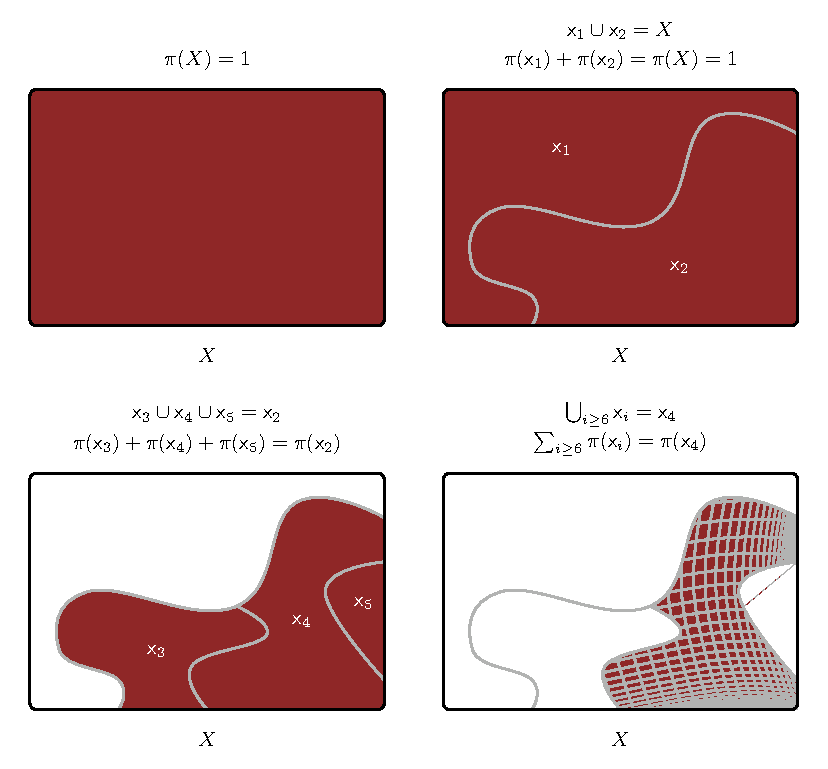
\includegraphics[width=0.75\textwidth,height=\textheight]{figures/distribution/distribution.pdf}

}

\caption{\label{fig-distribution}A probability distribution defines a
proportional allocation across a measurable space such that no matter
how we slice up the ambient set \(X\) into measurable subsets the total
probability is always preserved.}

\end{figure}

A set equipped with a \(\sigma\)-algebra and a probability distribution
is known as a \textbf{probability space}. Sometimes the combination
\((X, \mathcal{X}, \pi)\) is also known as a \textbf{probability
triple}.

Probability spaces are also sometimes denoted by \[
x \sim \pi,
\] where \(x \in X\) indicates the ambient set and a \(\sigma\)-algebra
is taken for granted. In words this reads ``the variable \(x\) is
distributed according to \(\pi\)'' or ``the variable \(x\) follows the
distribution \(\pi\)''. That said because probability distributions are
generally defined over measurable subsets and not individual elements a
more precise description be would be ``the variable \(x\) takes values
in a set \(X\) that is equipped with a probability distribution
\(\pi\)''. The emphasis on variables instead of spaces in this notation
is related to the awkward notion of a ``random variable'' which we will
discuss in more detail in Chapter Ten.

\hypertarget{derived-properties}{%
\subsection{Derived Properties}\label{derived-properties}}

Although these definitions might appear to be a bit stark, we can derive
all of the usual rules of measure and probability theory from them.

For example consider one measurable subset that is strictly smaller than
another, \[
\mathsf{x}_{1} \subset \mathsf{x}_{2} \in \mathcal{X}.
\] In this case we can always write \[
\mathsf{x}_{2} = \mathsf{x}_{1} \cup \mathsf{x}_{3}
\] for the non-empty, measurable subset of elements that are in
\(\mathsf{x}_{2}\) but not in \(\mathsf{x}_{1}\). Applying countable
additivity then gives \begin{align*}
\pi(\mathsf{x}_{2})
&= \pi(\mathsf{x}_{1} \cup \mathsf{x}_{3})
\\
&= \pi(\mathsf{x}_{1}) + \pi(\mathsf{x}_{3})
\\
&\ge \pi(\mathsf{x}_{1})
\end{align*} because \(\pi(\mathsf{x}_{3}) \ge 0\). In other words
larger measurable subsets are always allocated more or equal probability
than smaller subsets.

Similarly because any subset and its complement are disjoint and combine
to reconstruct the full set we always have \begin{align*}
1
&= \pi(X)
\\
&= \pi(\mathsf{x} \cup \mathsf{x}^{c})
\\
&= \pi(\mathsf{x}) + \pi(\mathsf{x}^{c})
\end{align*} or \[
\pi(\mathsf{x}^{c}) = 1 - \pi(\mathsf{x}).
\]

In order to work with two measurable subsets
\(\mathsf{x}_{1}, \mathsf{x}_{2} \in \mathcal{X}\) that might not be
disjoint (Figure~\ref{fig-disjoint-decomposition}) we have to consider
the elements that are unique to each, \[
\mathsf{x}_{1 \setminus 2}
=
\{ x \in X \mid x \in \mathsf{x}_{1}, x \notin \mathsf{x}_{2} \}
\] and \[
\mathsf{x}_{2 \setminus 1}
=
\{ x \in X \mid x \in \mathsf{x}_{2}, x \notin \mathsf{x}_{1} \},
\] and the elements that are shared, \[
\mathsf{x}_{1} \cap \mathsf{x}_{2}
=
\{ x \in X \mid x \in \mathsf{x}_{1}, x \in \mathsf{x}_{2} \}.
\]

\begin{figure}

\begin{minipage}[t]{0.20\linewidth}

{\centering 

~

}

\end{minipage}%
%
\begin{minipage}[t]{0.60\linewidth}

{\centering 

\raisebox{-\height}{

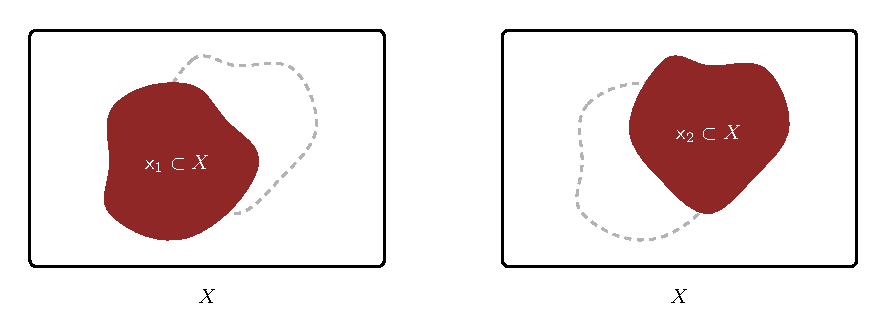
\includegraphics{figures/overlapping_sets/inputs/inputs.pdf}

}

}

\subcaption{\label{fig-input-subsets}}
\end{minipage}%
%
\begin{minipage}[t]{0.20\linewidth}

{\centering 

~

}

\end{minipage}%
\newline
\begin{minipage}[t]{0.05\linewidth}

{\centering 

~

}

\end{minipage}%
%
\begin{minipage}[t]{0.90\linewidth}

{\centering 

\raisebox{-\height}{

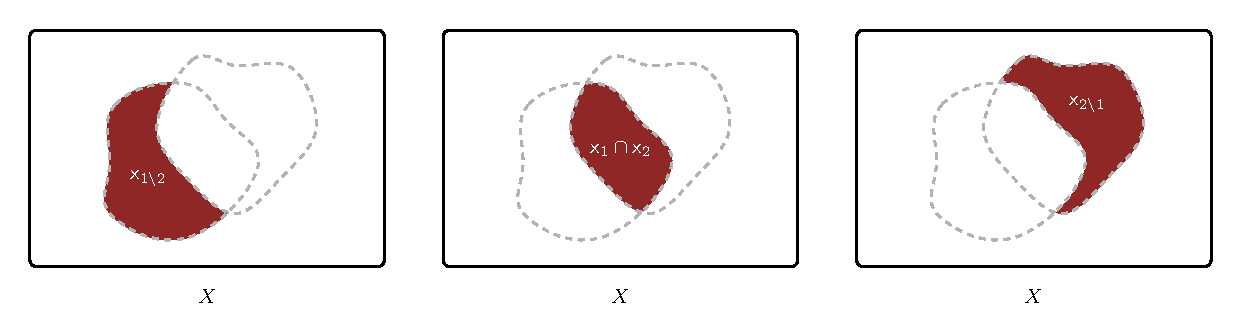
\includegraphics{figures/overlapping_sets/disjoint_components/disjoint_components.pdf}

}

}

\subcaption{\label{fig-disjoint-components}}
\end{minipage}%
%
\begin{minipage}[t]{0.05\linewidth}

{\centering 

~

}

\end{minipage}%

\caption{\label{fig-disjoint-decomposition}The union of (a) two
overlapping subsets \(\mathsf{x}_{1}\) and \(\mathsf{x}_{2}\) can always
be decomposed into the union of (b) three disjoint subsets. One disjoint
subset \(\mathsf{x}_{1 \setminus 2}\) encapsulates the elements unique
to \(\mathsf{x}_{1}\), another \(\mathsf{x}_{2 \setminus 1}\)
encapsulates the elements unique to \(\mathsf{x}_{2}\), and finally the
intersection \(\mathsf{x}_{1} \cap \mathsf{x}_{2}\) encapsulates the
elements shared by the two input subsets.}

\end{figure}

This then allows us to decompose \(\mathsf{x}_{1}\), \(\mathsf{x}_{2}\),
and their union into disjoint, measurable subsets
(Figure~\ref{fig-input-reconstruction},) \begin{align*}
\mathsf{x}_{1} &=
\mathsf{x}_{1 \setminus 2} \cup (\mathsf{x}_{1} \cap \mathsf{x}_{2})
\\
\mathsf{x}_{2} &=
\mathsf{x}_{2 \setminus 1} \cup (\mathsf{x}_{1} \cap \mathsf{x}_{2})
\\
\mathsf{x}_{1} \cup \mathsf{x}_{2} &=
\mathsf{x}_{1 \setminus 2}
\cup
( \mathsf{x}_{1} \cap \mathsf{x}_{2} )
\cup
\mathsf{x}_{2 \setminus 1}.
\end{align*}

\begin{figure}

{\centering 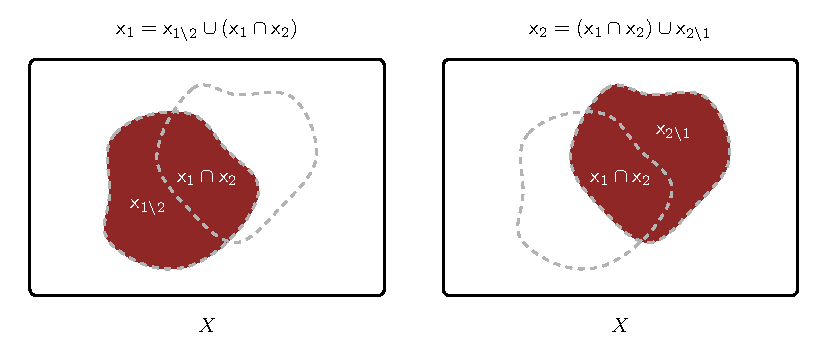
\includegraphics[width=0.6\textwidth,height=\textheight]{figures/overlapping_sets/input_reconstruction/input_reconstruction.pdf}

}

\caption{\label{fig-input-reconstruction}The disjoint subsets introduced
in (Figure~\ref{fig-disjoint-decomposition}) can also be used to
reconstruct the two input subsets individually.}

\end{figure}

Applying countable additivity to these three decompositions gives a
system of equations \begin{align*}
\pi(\mathsf{x}_{1}) &=
\pi(\mathsf{x}_{1 \setminus 2}) + \pi(\mathsf{x}_{1} \cap \mathsf{x}_{2})
\\
\pi(\mathsf{x}_{2}) &=
\pi(\mathsf{x}_{2 \setminus 1}) + \pi(\mathsf{x}_{1} \cap \mathsf{x}_{2})
\\
\pi(\mathsf{x}_{1} \cup \mathsf{x}_{2}) &=
\pi(\mathsf{x}_{1 \setminus 2})
+ \pi(\mathsf{x}_{1} \cap \mathsf{x}_{2})
+ \pi \mathsf{x}_{2 \setminus 1}).
\end{align*} Adding the first two together gives \[
\pi(\mathsf{x}_{1}) + \pi(\mathsf{x}_{2})
=
\pi(\mathsf{x}_{1 \setminus 2})
+ 2 \, \pi(\mathsf{x}_{1} \cap \mathsf{x}_{2})
+ \pi(\mathsf{x}_{1} \cap \mathsf{x}_{2})
\] or \[
\pi(\mathsf{x}_{1 \setminus 2})
+ \pi(\mathsf{x}_{1} \cap \mathsf{x}_{2})
+ \pi(\mathsf{x}_{1} \cap \mathsf{x}_{2})
=
\pi(\mathsf{x}_{1}) + \pi(\mathsf{x}_{2})
- \pi(\mathsf{x}_{1} \cap \mathsf{x}_{2}).
\] Substituting this into the third equation finally gives \[
\pi(\mathsf{x}_{1} \cup \mathsf{x}_{2})
=
\pi(\mathsf{x}_{1}) + \pi(\mathsf{x}_{2})
- \pi(\mathsf{x}_{1} \cap \mathsf{x}_{2}).
\]

\hypertarget{measures-and-probability-distributions-in-practice}{%
\subsection{Measures and Probability Distributions In
Practice}\label{measures-and-probability-distributions-in-practice}}

The formal definition of measures and probability distributions tell us
what form the consistent allocation of any quantity on any measurable
space has to take, but it does not necessarily provide a way for
constructing explicit allocations in practice. Specifically in almost
all circumstances it is infeasible, if not outright impossible, to
exhaustively specify the measure or probability allocated to
\emph{every} subset in the ambient \(\sigma\)-algebra. Constructing and
then storing infinitely large databases linking each measurable subset
to their allocations is not particularly practical!

In some cases we can define a useful measures and probability
distributions by specifying the allocation to only some of the
measurable subsets and then deriving the allocations to the rest with
countable additivity. For example in finite and countable spaces we need
to specify only the allocations to atomic subsets, and in some
uncountable spaces we might need to specify only the allocations to
certain nice subsets.

That said in most of these cases those reduced allocations are still
impractical to specify one-by-one. Because of that our introduction to
general measure and probability theory will have to remain a bit
abstract, without any explicit examples, for the time being.

In applied problems measures and probability distributions are almost
always defined \emph{algorithmically}, with rules to evaluate the
measure or probability allocated to a subset on the fly instead of
storing and retrieving the allocation from an exhaustive specification.
We will introduce two of the most important algorithm representations of
measures and probability distributions, and use them to define many
useful allocations, in Chapter Five and Chapter Eight.

\hypertarget{interpretations-of-measure-and-probability}{%
\section{Interpretations of Measure And
Probability}\label{interpretations-of-measure-and-probability}}

To this point our treatment of measure and probability theory has been
purely mathematical. A measures defines the allocations of some abstract
conserved quantity across some abstract measurable space; a probability
distribution defines a proportional allocations. This mathematical
construction cannot be endowed with any particular interpretation until
we use it to model something.

In this section we'll review some of the most common applications of
measure and probability theory and the particular interpretations those
applications create.

\hypertarget{modeling-physical-distributions}{%
\subsection{Modeling Physical
Distributions}\label{modeling-physical-distributions}}

One immediate application of measure theory is to model the behavior of
a physical quantity, such as mass or electric charge. For example
physical mass can be distributed across a solid object in a variety of
different ways, with the exact distribution affecting how that object
interacts with the surrounding environment. Similarly the distribution
of charge across the surface of a conducting object defines its
electrostatic properties.

In some physical systems the distribution can also change with time and
influence the dynamics of the system. Time-dependent measures that
quantify how the distribution of a physical quantity evolves are a
common feature of many mathematical physical theories.

\hypertarget{modeling-populations}{%
\subsection{Modeling Populations}\label{modeling-populations}}

A similar application is modeling the selection of individuals, or the
properties of individuals, from a larger population. Each time we
\emph{sample} a subset of individuals from the population we will
observe a different ensemble of behaviors, such as political or consumer
preferences, heights, or ages. The heterogeneity of these
characteristics across the population can often be quantified with
measures, and their relative occurrences modeled with probability
distributions.

For example is \(30\%\) of the individuals in a population have a height
between \(0\) feet and \(5\) feet then a probability distribution
modeling the variation in heights would give \[
\pi([0, 5]) = 0.3.
\]

\hypertarget{modeling-frequencies}{%
\subsection{Modeling Frequencies}\label{modeling-frequencies}}

An application particular to probability theory concerns the frequencies
of repeated events.

Consider an abstract event whose outcomes take \emph{unpredictable}
values in some space \(X\). Perfectly replicating the circumstances of
this event \(N\) times defines a sequence of values in \(Y\), \[
\{ x_{1}, \ldots, x_{n}, \ldots x_{N} \}.
\]

While we cannot predict what values the individual events in this
sequence will take, we may be able to characterize how often certain
outcomes appear relative to others. In particular we can define the
\textbf{frequency} of a subset \(\mathsf{x} \subset X\) by the number of
events that that take values in \(\mathsf{x}\), \[
f_{N}(\mathsf{x})
= \frac{ \sum_{n = 1}^{N} \mathbb{I}_{\mathsf{x}}(x_{n}) }{N},
\] where \[
\mathbb{I}_{\mathsf{x}}(x)
=
\left\{
\begin{array}{rr}
1, & x \in \mathsf{x} \\
0, & x \notin \mathsf{x}
\end{array}
\right. .
\]

Replicating the event a countably infinite number of times defines the
\textbf{asymptotic} or \textbf{long-run} frequency of a subset,
\begin{align*}
f(\mathsf{x})
&=
\lim_{N \rightarrow \infty} f_{N}(\mathsf{x})
\\
&=
\lim_{N \rightarrow \infty}
\frac{ \sum_{n = 1}^{N} \mathbb{I}_{\mathsf{x}}(x_{n}) }{N}.
\end{align*} In other words the more frequent subsets contain more
common event outcomes.

If the frequencies are the same for \emph{any} sequence of events then
we can model them with probability theory. Specifically we can interpret
the allocated probabilities as the proportion of the total event
outcomes that fall into each subset of outcome values.

In this case the particular ordering of the event sequences doesn't
matter and we can also interpret them as defining a population of
possible events. From this perspective the application of probability
theory is equivalent to the application in the previous section.

\hypertarget{modeling-uncertainties}{%
\subsection{Modeling Uncertainties}\label{modeling-uncertainties}}

Probability theory can also be used to consistently quantify uncertain
information.

Consider a space of possible statements \(X\). Under perfect knowledge
we would be able to specify a particular statement \(x \in X\) as true
with all other statements in \(X\) being false. In other words certainty
is quantified with binary true/false assignments. When our knowledge is
not quite so certain, however, we have to soften those claims.

To quantify uncertain information we have to generalize beyond binary
true/false assignments to continuous values that \emph{interpolate}
between absolute truth and falsity. The larger the value we assign to a
subset of statements the more our uncertain information supports one of
those statements being true. Conversely the smaller the value we assign
to a subset the more our uncertain information supports all of the
included statements being false.

Applying probability theory allows us to enforce consistent uncertainty
assignments across all of the possible statements. The individual
probability allocations can then be interpreted as quantifying how
strongly our information supports that one of the statements within a
measurable set is true. In this setting the allocated probabilities are
sometimes referred to as ``plausibilities'', ``credibilities'', and
``beliefs''.

For example the property that \(\pi(X) = 1\) corresponds to the fact
that at least one of the statements in \(X\) always has to be true. A
probability distribution that concentrates around the statement \(x\)
encodes confidence that one of the statements near \(x\) is true. The
singular limit where all of the available probability collapses onto a
single statement, \(\pi( \{ x \} ) = 1\), communicates certainty that
\(x\) is true.

This kind of probabilistic uncertainty quantification can be interpreted
in many ways. For example we can use it out model the personal,
subjective beliefs that an individual holds about the behavior of a
system. In particular we can use it to model our own specific beliefs.
At the same time we can use it to model the collective understanding of
entire communities. We can also use probability theory to model only
certain aspects of individual or community knowledge and not attempt to
quantify the entirety of that knowledge at once.

More formally this application defines one way to generalize classical
propositional logic to a many-valued logic. Using probability theory to
generalize other logical systems can sometimes also be possible,
although the technical details quickly become more complicated.

\hypertarget{everyone-play-nicely}{%
\subsection{Everyone Play Nicely}\label{everyone-play-nicely}}

A key point of confusion in probability theory is the confounding of its
abstract mathematical structure with the interpretations that arise in
particular applications. This confusion is made all the worse by the
long history of attempts to \emph{derive} probability theory from these
particular applications.

For example many have tried to derive probabilities as asymptotic
frequencies of physical events. The key motivations of this approach is
that the resulting probabilities would be objective in the sense that
everyone who could implement those infinite trials would attain the same
probabilities. Even if we ignore the impracticality of perfectly
repeating an event an infinite number of times within a finite lifetime
it turns out that there are also some subtle mathematical complications
with this approach. For a comprehensive discussion see Diaconis and
Skyrms (2017).

Similarly many have tried to derive probability theory from uncertainty
quantification. For example the Cox postulates (Van Horn, Kevin S.
(2003)) define basic intuitions about uncertainty quantification. On
simpler spaces these rules are equivalent to probability theory, but
that equivalence doesn't persist to more general spaces. Because of that
this approach is not able to recover the full generality of probability
theory.

A common reaction to these technical difficulties is to resort to a sort
of philosophical bait and switch. When one cannot derive probability
theory from a particular application one might define probability theory
abstractly, as we have done above, but then impose an \emph{arbitrary}
restriction that it can only ever be applied to that one application.
For example those trying to derive probability theory from frequencies
might argue that probability theory can be applied to model only
frequencies, in which case all probabilities are frequencies. Others
trying to derive probability theory from the Cox axioms might argue that
any application of probability theory always models uncertain
information.

These interpretational restrictions then force some awkward
philosophical contortions when trying to apply probability theory in
practice. For example after imposing that all probabilities are
frequencies the only way to model uncertainty in the value of some
quantity is to treat it as the outcome of some hypothetical, and
completely non-existent, event. The introduction of these hypothetical
events to real events makes the entire system more difficult to
understand.

In this book we will avoid these restrictions, respect the full
generality of probability theory, and take advantage of any consistent
applications that might be useful in a given problem. Indeed we will
often take advantage of multiple applications \emph{at the same time}.

Consider, for example, a binary space \(X = {0, 1}\) that corresponds to
the two sides of a coin. In particular let \texttt{0} denote tails and
\texttt{1} denote heads. Any probability distribution over \(X\) can be
quantified with the probability \(p \in [0, 1]\) allocated to the point
\texttt{1}, which gives the consistent probability allocations
\begin{align*}
\pi( \emptyset; p ) &= 0
\\
\pi( {0}; p ) &= 1 - p
\\
\pi( {1}; p ) &= p
\\
\pi( X; p ) &= 1.
\end{align*}

There are many ways to flip a coin, but let's say that we flip our coin
in a way that results in an unpredictable sequence of heads and tails.
The asymptotic frequencies of these outcomes can then be modeled with an
application of probability theory. In other words we can use a
probability distribution \(\pi(\cdot; p)\) to model the physical
outcomes of the flips.

At the same time we use probability theory to model any uncertainty in
which of the possible frequency models best matches the true behavior of
the coin. In particular we can construct a probability distribution over
the unit interval to quantify how compatible each probability allocation
\(p \in [0, 1]\) is with our knowledge of the coin.

If we have a bag of \(I\) coins then could also model the variation in
the probability parameters \[
\{ p_{1}, \ldots, p_{i}, \ldots, p_{I} \}
\] for each coin. In this case we can apply probability theory once
again, this time to model the population of coin behaviors.

To be clear the interpretations inherent to particular applications of
probability theory are important for ensuring that we implement those
applications correctly in practice. Elevating one interpretation to the
exclusion of others, however, excludes the corresponding applications
and limits the full potential of probability theory. To take full
advantage of the practical utility of probability theory we have to
respect all of consistent applications!

\hypertarget{conclusion}{%
\section{Conclusion}\label{conclusion}}

Conceptually measure and probability theory are straightforward. Measure
theory quantifies how we can consistently allocate a conserved quantify
across a general mathematical space and probability theory considers the
special case of proportional allocations. In order to quantify that
conceptual simplicity, however, we need to resort to some careful
mathematics. In particular we need to incorporate \(\sigma\)-algebras to
surgically remove any pathological behavior that can arise, even on
seemingly well-behaved spaces such as the real line, and obstruct
consistent allocations.

Once we've safely constructed these theories in full generality we can
use the apply abstract mathematics to model particular systems. Within
these applications the math inherits particular interpretations, but we
have to be careful to not take these circumstantial interpretations too
seriously lest we abandon the full utility of the abstract mathematics.

The technical exploration of measures and probability distributions goes
far beyond the introduction in this chapter. Unfortunately many
textbooks that cover this material can be difficult to parse without
extensive mathematical experience. My personal favorite is Folland
(1999) which, while technically rigorous, provides more exposition and
motivation than I have found in other treatments.

\hypertarget{acknowledgements}{%
\section{Acknowledgements}\label{acknowledgements}}

I thank Jeff Helzner for helpful discussion.

A very special thanks to everyone supporting me on Patreon: Adam
Fleischhacker, Adriano Yoshino, Alan Chang, Alessandro Varacca,
Alexander Bartik, Alexander Noll, Alexander Petrov, Alexander Rosteck,
Anders Valind, Andrea Serafino, Andrew Mascioli, Andrew Rouillard,
Andrew Vigotsky, Angie\_Hyunji Moon, Ara Winter, Austin Rochford, Austin
Rochford, Avraham Adler, Ben Matthews, Ben Swallow, Benjamin Glemain,
Bradley Kolb, Brandon Liu, Brynjolfur Gauti Jónsson, Cameron Smith,
Canaan Breiss, Cat Shark, Charles Naylor, Chase Dwelle, Chris Jones,
Chris Zawora, Christopher Mehrvarzi, Colin Carroll, Colin McAuliffe,
Damien Mannion, Damon Bayer, dan mackinlay, Dan Muck, Dan W Joyce, Dan
Waxman, Dan Weitzenfeld, Daniel Edward Marthaler, Darshan Pandit,
Darthmaluus , David Burdelski, David Galley, David Wurtz, Doug Rivers,
Dr.~Jobo, Dr.~Omri Har Shemesh, Ed Cashin, Edgar Merkle, Eric LaMotte,
Erik Banek, Ero Carrera, Eugene O'Friel, Felipe González, Fergus
Chadwick, Finn Lindgren, Florian Wellmann, Francesco Corona, Geoff
Rollins, Granville Matheson, Greg Sutcliffe, Guido Biele, Hamed
Bastan-Hagh, Haonan Zhu, Hector Munoz, Henri Wallen, hs, Hugo Botha,
Håkan Johansson, Ian Costley, Ian Koller, idontgetoutmuch, Ignacio Vera,
Ilaria Prosdocimi, Isaac Vock, J, J Michael Burgess, Jair Andrade, James
Hodgson, James McInerney, James Wade, Janek Berger, Jason Martin, Jason
Pekos, Jason Wong, Jeff Burnett, Jeff Dotson, Jeff Helzner, Jeffrey
Erlich, Jesse Wolfhagen, Jessica Graves, Joe Wagner, John Flournoy,
Jonathan H. Morgan, Jonathon Vallejo, Joran Jongerling, Joseph Despres,
Josh Weinstock, Joshua Duncan, Joshua Griffith, JU, Justin Bois, Karim
Naguib, Karim Osman, Kejia Shi, Kevin Foley, Kristian Gårdhus Wichmann,
Kádár András, Lars Barquist, lizzie , LOU ODETTE, Marc Dotson, Marcel
Lüthi, Marek Kwiatkowski, Mark Donoghoe, Markus P., Martin Modrák, Matt
Moores, Matthew, Matthew Kay, Matthieu LEROY, Maurits van der Meer,
Merlin Noel Heidemanns, Michael DeWitt, Michael Dillon, Michael Lerner,
Mick Cooney, Márton Vaitkus, N Sanders, Name, Nathaniel Burbank, Nic
Fishman, Nicholas Clark, Nicholas Cowie, Nick S, Nicolas Frisby, Octavio
Medina, Ole Rogeberg, Oliver Crook, Olivier Ma, Pablo León Villagrá,
Patrick Kelley, Patrick Boehnke, Pau Pereira Batlle, Peter Smits, Pieter
van den Berg , ptr, Putra Manggala, Ramiro Barrantes Reynolds, Ravin
Kumar, Raúl Peralta Lozada, Riccardo Fusaroli, Richard Nerland, Robert
Frost, Robert Goldman, Robert kohn, Robert Mitchell V, Robin Taylor,
Ross McCullough, Ryan Grossman, Rémi , S Hong, Scott Block, Sean
Pinkney, Sean Wilson, Seth Axen, shira, Simon Duane, Simon Lilburn,
sssz, Stan\_user, Stefan, Stephanie Fitzgerald, Stephen Lienhard, Steve
Bertolani, Stew Watts, Stone Chen, Susan Holmes, Svilup, Sören Berg, Tao
Ye, Tate Tunstall, Tatsuo Okubo, Teresa Ortiz, Thomas Lees, Thomas
Vladeck, Tiago Cabaço, Tim Radtke, Tobychev , Tom McEwen, Tony Wuersch,
Utku Turk, Virginia Fisher, Vitaly Druker, Vladimir Markov, Wil
Yegelwel, Will Farr, Will Tudor-Evans, woejozney, yolhaj , yureq , Zach
A, Zad Rafi, and Zhengchen Cai.

\hypertarget{references}{%
\section*{References}\label{references}}
\addcontentsline{toc}{section}{References}

\hypertarget{refs}{}
\begin{CSLReferences}{1}{0}
\leavevmode\vadjust pre{\hypertarget{ref-DiaconisEtAl:2017}{}}%
Diaconis, Persi, and Brian Skyrms. 2017. \emph{Ten Great Ideas about
Chance}. Princeton University Press.

\leavevmode\vadjust pre{\hypertarget{ref-Folland:1999}{}}%
Folland, G. B. 1999. \emph{Real Analysis: Modern Techniques and Their
Applications}. New York: John Wiley; Sons, Inc.

\leavevmode\vadjust pre{\hypertarget{ref-VanHorn:2003}{}}%
Van Horn, Kevin S. 2003. {``{Constructing a logic of plausible
inference: a guide to {C}ox's theorem}.''} \emph{{International Journal
of Approximate Reasoning}} 34 (1): 3--24.

\end{CSLReferences}

\hypertarget{license}{%
\section*{License}\label{license}}
\addcontentsline{toc}{section}{License}

A repository containing all of the files used to generate this chapter
is available on
\href{https://github.com/betanalpha/quarto_chapters/tree/main/probability_on_general_spaces}{GitHub}.

The text and figures in this chapter are copyrighted by Michael
Betancourt and licensed under the CC BY-NC 4.0 license:

https://creativecommons.org/licenses/by-nc/4.0/



\end{document}
